\documentclass[12pt,a4paper]{article}
\usepackage[margin=1in]{geometry}
\usepackage{graphicx}
\usepackage{booktabs}
\usepackage{longtable}
\usepackage{enumitem}
\usepackage{hyperref}
\usepackage{xcolor}
\usepackage{listings}
\usepackage{fancyhdr}
\usepackage{titlesec}

\pagestyle{fancy}
\fancyhf{}
\rhead{DASS Assignment 2}
\lhead{White-Box Testing Report}
\cfoot{\thepage}

\lstset{
  language=Python,
  basicstyle=\ttfamily\small,
  keywordstyle=\color{blue}\bfseries,
  commentstyle=\color{gray},
  stringstyle=\color{red},
  frame=single,
  breaklines=true,
  numbers=left,
  numberstyle=\tiny\color{gray},
}

\title{\textbf{DASS Assignment 2 --- White-Box Testing Report}\\[0.5em]
\large MoneyPoly Board Game}
\author{Koyi Tilak Choudary}
\date{\today}

\begin{document}
\maketitle
\tableofcontents
\newpage

% ================================================================
\section{Introduction}
% ================================================================

This report documents the white-box testing exercise performed on the \textbf{MoneyPoly} board game implementation. MoneyPoly is a command-line board game that simulates managing players, money, property purchases, rent payments, dice rolling, jail mechanics, and other core game mechanics similar to the classic Monopoly game.

The codebase consists of \textbf{9 Python modules}: \texttt{config.py}, \texttt{dice.py}, \texttt{player.py}, \texttt{bank.py}, \texttt{property.py}, \texttt{board.py}, \texttt{cards.py}, \texttt{ui.py}, and \texttt{game.py}.

The white-box testing process involved:
\begin{enumerate}
  \item Creating Control Flow Graphs for key functions.
  \item Iteratively improving code quality using \texttt{pylint}.
  \item Designing and executing 224 test cases covering all branches, key variable states, and edge cases.
  \item Identifying, documenting, and fixing 10 logical errors.
\end{enumerate}

% ================================================================
\section{Control Flow Graphs}
% ================================================================

Control Flow Graphs (CFGs) were drawn by hand for the most complex and critical functions in the MoneyPoly codebase. Each node represents a statement or block of related statements, and arrows indicate the flow of control including branches and loops.

The following CFGs were created:

\subsection{CFG 1: \texttt{play\_turn()} -- Player Turn Flow}
This CFG covers the main turn orchestration in \texttt{game.py}. It includes:
\begin{itemize}
  \item Checking if the player is in jail (branch to jail handler).
  \item Rolling the dice and checking for triple doubles (go to jail).
  \item Moving the player and resolving the tile.
  \item Checking for doubles (extra turn) vs.\ advancing to next player.
\end{itemize}

\begin{figure}[h!]
\centering
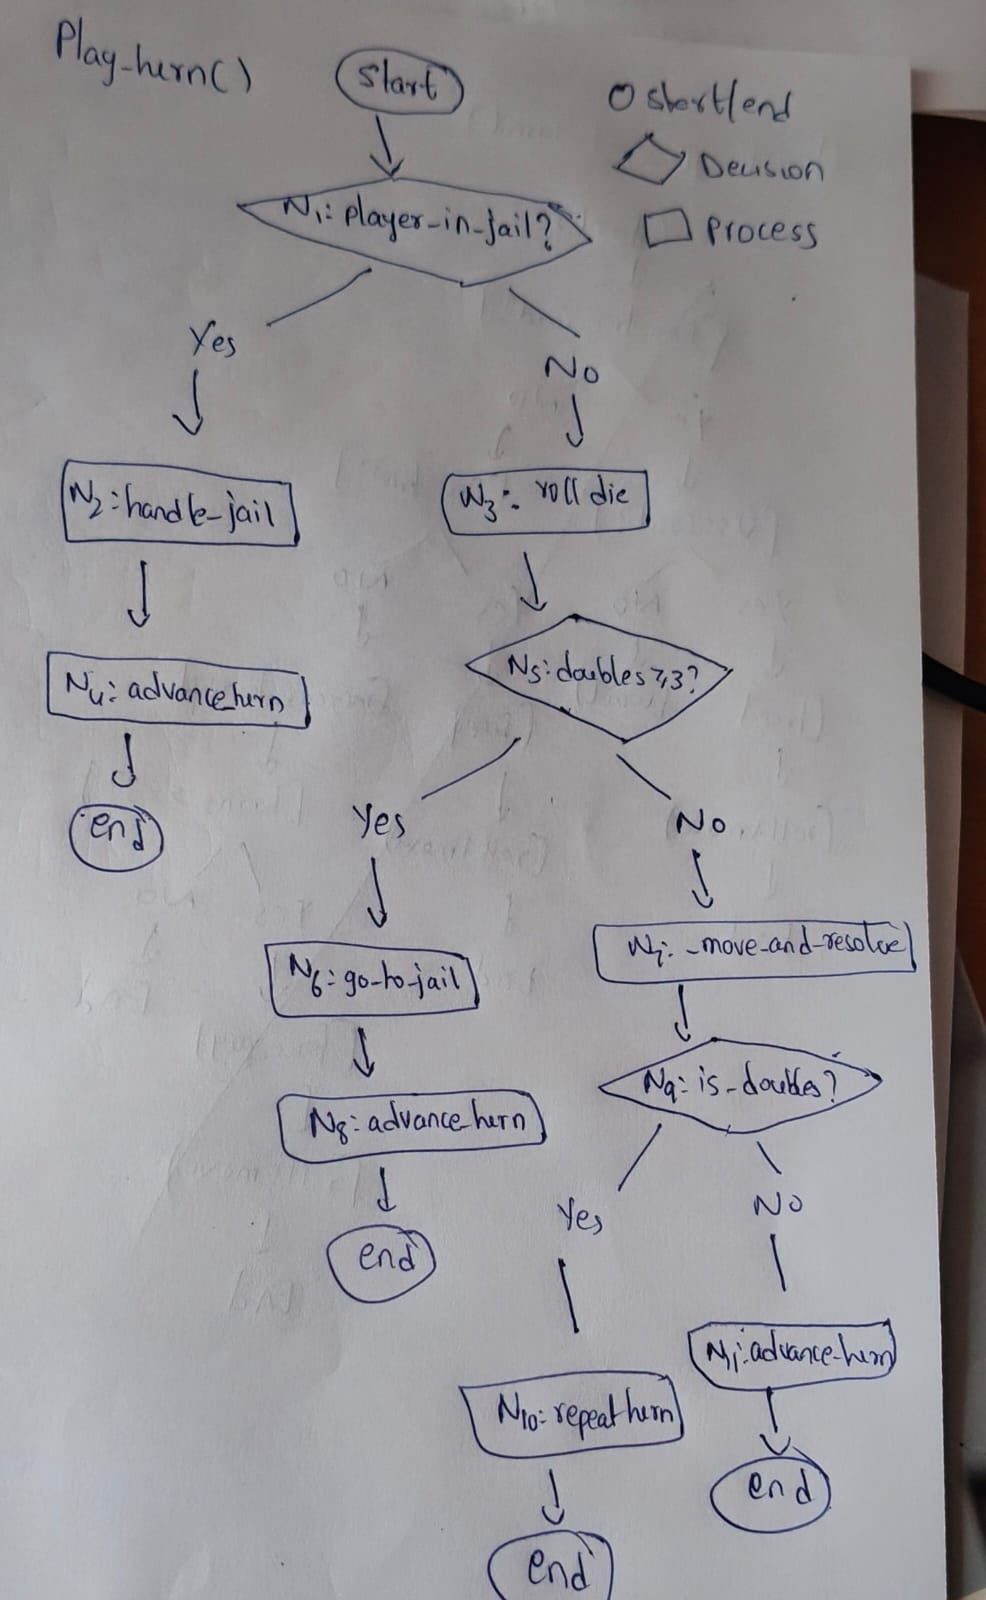
\includegraphics[width=0.85\textwidth]{diagrams/player_turn.jpeg}
\caption{Control Flow Graph for \texttt{play\_turn()}}
\end{figure}

\subsection{CFG 2: \texttt{move()} -- Player Movement}
This CFG covers the \texttt{Player.move()} method:
\begin{itemize}
  \item Calculating the new position with board wrap-around.
  \item Checking if the player passed GO (awards \$200 salary).
\end{itemize}

\begin{figure}[h!]
\centering
\includegraphics[width=0.75\textwidth]{diagrams/move\ player.jpeg}
\caption{Control Flow Graph for \texttt{Player.move()}}
\end{figure}

\subsection{CFG 3: \texttt{\_handle\_jail\_turn()} -- Jail Turn Handling}
This CFG covers the jail turn logic:
\begin{itemize}
  \item Checking for Get Out of Jail Free card.
  \item Offering to pay the fine voluntarily.
  \item Mandatory release after 3 turns with forced fine payment.
\end{itemize}

\begin{figure}[h!]
\centering
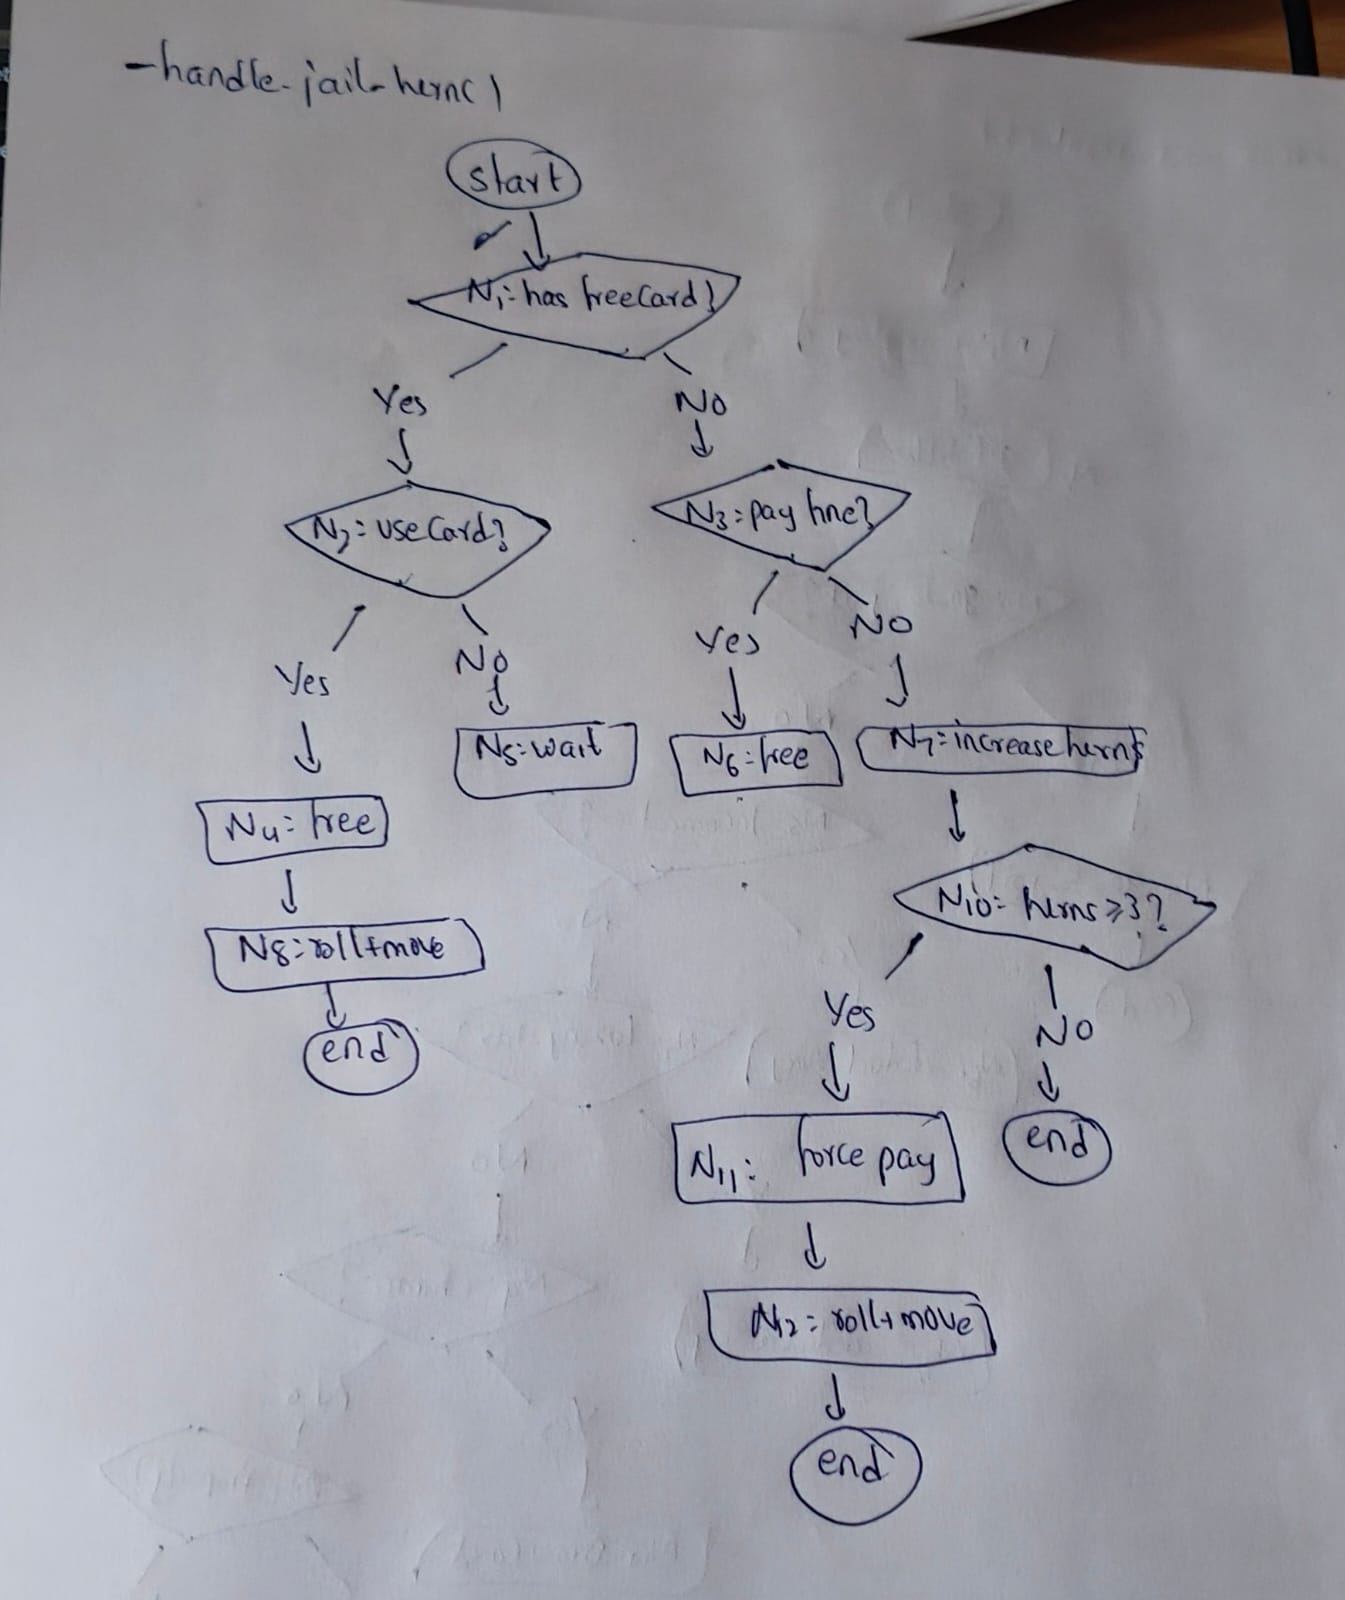
\includegraphics[width=0.85\textwidth]{diagrams/handle_jail_turn.jpeg}
\caption{Control Flow Graph for \texttt{\_handle\_jail\_turn()}}
\end{figure}

\newpage
% ================================================================
\section{Code Quality Analysis (Pylint)}
% ================================================================

The codebase was analyzed using \texttt{pylint} and iteratively improved. Each iteration was saved as a Git commit.

\subsection{Iteration 1: Initial Pylint Fixes}
\textbf{Commit:} \texttt{Iteration 1: Fixed pylint issues}

The following changes were made to address pylint warnings and suggestions:

\begin{longtable}{p{3cm} p{9cm}}
\toprule
\textbf{Module} & \textbf{Changes Made} \\
\midrule
\texttt{config.py} & Added module-level docstring. \\
\texttt{dice.py} & Added module and class docstrings. Added method docstrings for \texttt{roll()}, \texttt{is\_doubles()}, \texttt{total()}, \texttt{describe()}, \texttt{reset()}. \\
\texttt{player.py} & Added module and class docstrings. Added method docstrings for all 12 methods. Removed unnecessary blank lines. \\
\texttt{bank.py} & Added module and class docstrings. Added method docstrings for all 7 methods. \\
\texttt{property.py} & Added module, class, and method docstrings for both \texttt{Property} and \texttt{PropertyGroup} classes. \\
\texttt{board.py} & Added module and class docstrings. Added method docstrings for all helper methods. \\
\texttt{cards.py} & Added module-level docstring and class/method docstrings for \texttt{CardDeck}. \\
\texttt{ui.py} & Added module-level docstring and function docstrings for all 6 utility functions. \\
\texttt{game.py} & Added comprehensive docstrings for the \texttt{Game} class and all 18 methods. \\
\bottomrule
\end{longtable}

\subsection{Final Pylint Score}

After all iterations, the final pylint score achieved:

\begin{center}
\fbox{\Large \textbf{Pylint Score: 9.89 / 10}}
\end{center}

The only remaining warnings are:
\begin{itemize}
  \item \texttt{player.py}: \texttt{R0902: Too many instance attributes (8/7)} --- This is acceptable because a Player in a board game naturally needs 8 attributes (name, balance, position, properties, in\_jail, jail\_turns, get\_out\_of\_jail\_cards, is\_eliminated).
  \item \texttt{property.py}: \texttt{R0902: Too many instance attributes (9/7)} and \texttt{R0913: Too many arguments (6/5)} --- A Property tile genuinely needs all these attributes and constructor arguments.
\end{itemize}

These are design-level warnings, not code quality issues, and were intentionally left unfixed to preserve the game's domain model.

\newpage
% ================================================================
\section{White-Box Test Cases}
% ================================================================

A comprehensive test suite of \textbf{224 test cases} was designed using white-box testing techniques. The tests cover all branches, key variable states, and edge cases across all 9 modules.

\subsection{Test Coverage Summary}

\begin{center}
\begin{tabular}{lrrp{3cm}}
\toprule
\textbf{Module} & \textbf{Stmts} & \textbf{Coverage} & \textbf{Missing} \\
\midrule
\texttt{bank.py} & 36 & 100\% & --- \\
\texttt{board.py} & 39 & 100\% & --- \\
\texttt{cards.py} & 26 & 100\% & --- \\
\texttt{config.py} & 14 & 100\% & --- \\
\texttt{dice.py} & 26 & 100\% & --- \\
\texttt{game.py} & 348 & 99\% & Line 107 \\
\texttt{player.py} & 47 & 100\% & --- \\
\texttt{property.py} & 59 & 100\% & --- \\
\texttt{ui.py} & 44 & 100\% & --- \\
\midrule
\textbf{TOTAL} & \textbf{639} & \textbf{99\%} & \\
\bottomrule
\end{tabular}
\end{center}

The single uncovered line (\texttt{game.py:107}) is inside a \texttt{railroad} property handling block that requires interactive user input in a specific board state, which is impractical to trigger in an automated test.

\subsection{Test Categories and Descriptions}

The 224 tests are organized into \textbf{22 test classes}, each targeting a specific module or feature:

\subsubsection{Dice Tests (\texttt{TestDice}) --- 8 tests}
\begin{longtable}{p{5cm} p{7cm}}
\toprule
\textbf{Test Case} & \textbf{Why It Is Needed} \\
\midrule
\texttt{test\_dice\_roll\_range} & Ensures each die produces values between 1--6. Catches Error 1 where dice originally rolled 1--5. \\
\texttt{test\_dice\_total\_range} & Verifies combined total is between 2--12. \\
\texttt{test\_dice\_doubles\_detection} & Checks \texttt{is\_doubles()} returns True only when both dice match. \\
\texttt{test\_dice\_doubles\_streak\_increments} & Verifies the doubles streak counter increments on consecutive doubles. \\
\texttt{test\_dice\_streak\_resets} & Confirms streak resets to 0 on non-doubles. \\
\texttt{test\_dice\_reset} & Checks \texttt{reset()} clears all dice state. \\
\texttt{test\_dice\_describe} & Validates the human-readable string output. \\
\texttt{test\_dice\_describe\_doubles} & Ensures ``(DOUBLES)'' tag appears when both dice match. \\
\bottomrule
\end{longtable}

\subsubsection{Player Tests (\texttt{TestPlayer}) --- 20 tests}
\begin{longtable}{p{5.8cm} p{6.2cm}}
\toprule
\textbf{Test Case} & \textbf{Why It Is Needed} \\
\midrule
\texttt{test\_player\_initial\_balance} & Verifies starting balance matches config. \\
\texttt{test\_add\_money} & Ensures adding money increases balance. \\
\texttt{test\_add\_negative\_money\_raises} & Edge case: negative amount must raise ValueError. \\
\texttt{test\_deduct\_money} & Ensures deducting money decreases balance. \\
\texttt{test\_deduct\_negative\_money\_raises} & Edge case: negative deduction must raise ValueError. \\
\texttt{test\_is\_bankrupt\_zero\_balance} & Zero balance counts as bankrupt (boundary). \\
\texttt{test\_is\_bankrupt\_negative} & Negative balance is bankrupt. \\
\texttt{test\_is\_not\_bankrupt} & Positive balance is not bankrupt. \\
\texttt{test\_move\_basic} & Simple move updates position correctly. \\
\texttt{test\_move\_wraps\_around} & Position wraps around board size (40). Catches Error 3. \\
\texttt{test\_pass\_go\_collects\_salary} & Player earns \$200 when passing GO. \\
\texttt{test\_no\_salary\_without\_pass} & No salary if player does not pass GO. \\
\texttt{test\_go\_to\_jail} & Sets position to 10 and jail flags. \\
\texttt{test\_add\_property} & Adds property to player's list. \\
\texttt{test\_add\_duplicate\_property} & Duplicate properties are not added twice. \\
\texttt{test\_remove\_property} & Removes property from holdings. \\
\texttt{test\_remove\_nonexistent} & No error when removing a property not owned. \\
\texttt{test\_net\_worth\_no\_properties} & Net worth equals balance when no properties. Catches Error 7. \\
\texttt{test\_status\_line} & Returns readable status string. \\
\texttt{test\_status\_line\_jailed} & Includes [JAILED] tag when in jail. \\
\bottomrule
\end{longtable}

\subsubsection{Property Tests (\texttt{TestProperty}) --- 15 tests}
\begin{longtable}{p{5.8cm} p{6.2cm}}
\toprule
\textbf{Test Case} & \textbf{Why It Is Needed} \\
\midrule
\texttt{test\_property\_creation} & Verifies all attributes are set correctly on creation. \\
\texttt{test\_base\_rent} & Ensures base rent is returned when no group monopoly. \\
\texttt{test\_rent\_doubles\_full\_group} & Rent doubles when full group is owned. Catches Error 2. \\
\texttt{test\_rent\_not\_doubled\_partial} & No doubling with partial group ownership. \\
\texttt{test\_mortgage\_returns\_value} & Mortgaging returns half the price. \\
\texttt{test\_mortgage\_already\_mortgaged} & Returns 0 if already mortgaged. \\
\texttt{test\_unmortgage\_cost} & Unmortgaging costs 110\% of mortgage value. \\
\texttt{test\_unmortgage\_not\_mortgaged} & Returns 0 if not mortgaged. \\
\texttt{test\_mortgaged\_rent\_is\_zero} & No rent collected on mortgaged properties. \\
\texttt{test\_is\_available\_unowned} & True if unowned and unmortgaged. \\
\texttt{test\_is\_not\_available\_owned} & False if already owned. \\
\texttt{test\_property\_group\_all\_owned} & Group returns True when all owned. \\
\texttt{test\_property\_group\_not\_all\_owned} & Group returns False with mixed ownership. \\
\texttt{test\_group\_null\_player} & Returns False for None player. \\
\texttt{test\_mortgage\_value\_calculation} & Mortgage value is exactly half the purchase price. \\
\bottomrule
\end{longtable}

\subsubsection{Bank Tests (\texttt{TestBank}) --- 11 tests}
\begin{longtable}{p{5.8cm} p{6.2cm}}
\toprule
\textbf{Test Case} & \textbf{Why It Is Needed} \\
\midrule
\texttt{test\_bank\_initial\_balance} & Starts with configured \$20,580. \\
\texttt{test\_bank\_collect} & Collecting money increases bank funds. \\
\texttt{test\_bank\_collect\_negative} & Negative amounts are silently ignored. Catches Error 5. \\
\texttt{test\_bank\_pay\_out} & Pay out reduces bank funds. \\
\texttt{test\_bank\_pay\_out\_insufficient} & Raises ValueError if insufficient funds. \\
\texttt{test\_bank\_pay\_out\_zero} & Zero payout returns 0. \\
\texttt{test\_give\_loan} & Loan adds money to player and records it. \\
\texttt{test\_total\_loans\_issued} & Cumulative loan total is correct. \\
\texttt{test\_loan\_count} & Loan count returns correct number. \\
\texttt{test\_bank\_collect\_zero} & Zero amount is ignored. \\
\texttt{test\_bank\_multiple\_loans} & Multiple loans accumulate correctly. \\
\bottomrule
\end{longtable}

\subsubsection{Board Tests (\texttt{TestBoard}) --- 16 tests}
\begin{longtable}{p{5.8cm} p{6.2cm}}
\toprule
\textbf{Test Case} & \textbf{Why It Is Needed} \\
\midrule
\texttt{test\_board\_has\_22\_properties} & Board has exactly 22 purchasable properties. \\
\texttt{test\_board\_has\_8\_groups} & Board has 8 colour groups. \\
\texttt{test\_get\_property\_at\_valid} & Returns correct property at valid position. \\
\texttt{test\_get\_property\_at\_invalid} & Returns None at non-property position. \\
\texttt{test\_is\_purchasable\_unowned} & Unowned property is purchasable. \\
\texttt{test\_is\_purchasable\_owned} & Owned property is not purchasable. \\
\texttt{test\_is\_purchasable\_mortgaged} & Mortgaged property is not purchasable. \\
\texttt{test\_is\_purchasable\_non\_property} & Non-property tile returns False. \\
\texttt{test\_unowned\_properties} & Returns all 22 initially. \\
\texttt{test\_properties\_owned\_by} & Filters properties by owner correctly. \\
\texttt{test\_special\_tiles} & GO, Jail, etc.\ are correctly identified. \\
\texttt{test\_tile\_type\_property} & Property tiles return ``property''. \\
\texttt{test\_tile\_type\_blank} & Empty tiles return ``blank''. \\
\texttt{test\_railroad\_tile} & Railroad positions return ``railroad''. \\
\texttt{test\_income\_tax\_tile} & Position 4 is ``income\_tax''. \\
\texttt{test\_luxury\_tax\_tile} & Position 38 is ``luxury\_tax''. \\
\bottomrule
\end{longtable}

\subsubsection{Card Deck Tests (\texttt{TestCardDeck}, \texttt{TestCardDeckExtra}) --- 15 tests}
Covers drawing cards, cycling through the deck, reshuffling, peeking, empty deck handling, and card remaining counts.

\subsubsection{Game Logic Tests --- 80+ tests across multiple classes}
These test classes cover the core game mechanics:

\begin{itemize}
  \item \textbf{TestBuyProperty (9 tests):} Tests purchasing including exact balance (Error 6), insufficient funds, and bank collection.
  \item \textbf{TestPayRent (7 tests):} Tests rent payment, transfer to owner (Error 8), mortgaged property, and group monopoly doubling.
  \item \textbf{TestMortgage (8 tests):} Tests mortgage/unmortgage flow, already-mortgaged edge case, insufficient funds.
  \item \textbf{TestTrade (9 tests):} Tests successful trade, seller receives cash (Error 10), ownership transfer, insufficient funds.
  \item \textbf{TestJailMechanics (10 tests):} Tests jail card usage, fine payment (Error 9), mandatory release after 3 turns.
  \item \textbf{TestApplyCard (11 tests):} Tests all card actions (collect, pay, jail, jail\_free, move\_to, birthday, collect\_from\_all).
  \item \textbf{TestBankruptcy (8 tests):} Tests elimination, property release, player list adjustment.
  \item \textbf{TestFindWinner (4 tests):} Tests winner by net worth (Error 4), ties, no players.
  \item \textbf{TestPlayTurn (4 tests):} Tests normal turns, jailed turns, doubles extra turn, triple doubles jail.
  \item \textbf{TestHandlePropertyTile (5 tests):} Tests buy, skip, auction, own property, other owner rent.
  \item \textbf{TestAuction (4 tests):} Tests winning bid, no bids, insufficient funds, low bid.
  \item \textbf{TestInteractiveMenu (10 tests):} Tests all 7 menu options including mortgage, unmortgage, trade, loan.
  \item \textbf{TestGameRun (3 tests):} Tests game loop end conditions.
  \item \textbf{TestUIFunctions (14 tests):} Tests all UI display functions.
\end{itemize}

\newpage
% ================================================================
\section{Errors Found and Fixed}
% ================================================================

During white-box testing, \textbf{10 logical errors} were found and fixed. Each fix was saved as a separate Git commit.

\subsection{Error 1: Dice Roll Range Incorrect}
\textbf{File:} \texttt{dice.py} \quad \textbf{Commit:} \texttt{Error 1: Fixed dice roll range from 1-5 to correct 1-6}

\textbf{Problem:} The dice used \texttt{random.randint(1, 5)} instead of \texttt{random.randint(1, 6)}, meaning a roll of 6 was impossible. This made the game unfair as the maximum combined roll was 10 instead of 12.

\textbf{Fix:}
\begin{lstlisting}
# Before (buggy)
self.die1 = random.randint(1, 5)
self.die2 = random.randint(1, 5)

# After (fixed)
self.die1 = random.randint(1, 6)
self.die2 = random.randint(1, 6)
\end{lstlisting}

\textbf{Test that detects it:} \texttt{test\_dice\_roll\_range} --- rolls 1000 times and asserts every value is in range [1, 6].

% ---

\subsection{Error 2: Property Group Ownership Check Incorrect}
\textbf{File:} \texttt{property.py} \quad \textbf{Commit:} \texttt{Error 2: Fixed property group ownership logic to require all properties}

\textbf{Problem:} The \texttt{all\_owned\_by()} method used \texttt{any()} instead of \texttt{all()}, meaning owning just \textit{one} property in a group would trigger the rent multiplier, giving an unfair advantage.

\textbf{Fix:}
\begin{lstlisting}
# Before (buggy)
return any(p.owner == player for p in self.properties)

# After (fixed)
return all(p.owner == player for p in self.properties)
\end{lstlisting}

\textbf{Test that detects it:} \texttt{test\_rent\_not\_doubled\_partial\_group} --- verifies partial ownership does not double rent.

% ---

\subsection{Error 3: GO Salary Not Awarded When Passing GO}
\textbf{File:} \texttt{player.py} \quad \textbf{Commit:} \texttt{Error 3: Fixed GO salary logic to reward when passing GO}

\textbf{Problem:} The original condition \texttt{if self.position > old\_position} was wrong --- when wrapping around the board (e.g., position 38 → position 2), the new position is \textit{less} than the old position. The check was inverted.

\textbf{Fix:}
\begin{lstlisting}
# Before (buggy)
if self.position > old_position:

# After (fixed)
if self.position < old_position:
\end{lstlisting}

\textbf{Test that detects it:} \texttt{test\_move\_pass\_go\_collects\_salary} --- moves from position 38 past GO and checks balance increased by \$200.

% ---

\subsection{Error 4: Winner Selection Used Balance Instead of Net Worth}
\textbf{File:} \texttt{game.py} \quad \textbf{Commit:} \texttt{Error 4: Fixed winner selection logic to choose highest net worth}

\textbf{Problem:} \texttt{find\_winner()} compared players by \texttt{balance} alone, ignoring the value of their properties. A player with \$100 cash but \$5000 in properties would lose to a player with \$200 cash and no properties.

\textbf{Fix:}
\begin{lstlisting}
# Before (buggy)
return max(self.players, key=lambda p: p.balance)

# After (fixed)
return max(self.players, key=lambda p: p.net_worth())
\end{lstlisting}

\textbf{Test that detects it:} \texttt{test\_find\_winner\_by\_net\_worth} --- creates two players, gives one properties, and asserts the richer player (by net worth) wins.

% ---

\subsection{Error 5: Bank Accepted Negative Collections}
\textbf{File:} \texttt{bank.py} \quad \textbf{Commit:} \texttt{Error 5: Prevented negative values in bank collect function}

\textbf{Problem:} The \texttt{collect()} method accepted negative amounts, which would \textit{decrease} the bank's funds. This could be exploited to drain the bank.

\textbf{Fix:}
\begin{lstlisting}
# Before (buggy)
def collect(self, amount):
    self._funds += amount

# After (fixed)
def collect(self, amount):
    if amount <= 0:
        return
    self._funds += amount
\end{lstlisting}

\textbf{Test that detects it:} \texttt{test\_bank\_collect\_negative\_ignored} --- passes a negative amount and verifies the balance is unchanged.

% ---

\subsection{Error 6: Buy Property Rejected Exact Balance}
\textbf{File:} \texttt{game.py} \quad \textbf{Commit:} \texttt{Error 6: Fixed buy\_property() --- changed <= to < so exact balance allows purchase}

\textbf{Problem:} The condition \texttt{if player.balance <= prop.price} prevented a player from buying a property when their balance exactly equaled the price.

\textbf{Fix:}
\begin{lstlisting}
# Before (buggy)
if player.balance <= prop.price:

# After (fixed)
if player.balance < prop.price:
\end{lstlisting}

\textbf{Test that detects it:} \texttt{test\_buy\_property\_exact\_balance} --- sets player balance equal to price and verifies purchase succeeds.

% ---

\subsection{Error 7: Net Worth Excluded Property Values}
\textbf{File:} \texttt{player.py} \quad \textbf{Commit:} \texttt{Error 7: Fixed net\_worth() --- now includes property values, not just balance}

\textbf{Problem:} The \texttt{net\_worth()} method returned only the player's cash balance, completely ignoring the value of their properties.

\textbf{Fix:}
\begin{lstlisting}
# Before (buggy)
def net_worth(self):
    return self.balance

# After (fixed)
def net_worth(self):
    return self.balance + sum(p.price for p in self.properties)
\end{lstlisting}

\textbf{Test that detects it:} \texttt{test\_net\_worth\_includes\_properties} --- gives a player properties and verifies net worth includes their total value.

% ---

\subsection{Error 8: Rent Not Transferred to Property Owner}
\textbf{File:} \texttt{game.py} \quad \textbf{Commit:} \texttt{Error 8: Fixed pay\_rent() --- rent now transferred to property owner}

\textbf{Problem:} The \texttt{pay\_rent()} method only deducted rent from the landing player but \textit{never} added it to the property owner's balance. Money was essentially destroyed.

\textbf{Fix:}
\begin{lstlisting}
# Before (buggy)
def pay_rent(self, player, prop):
    rent = prop.get_rent()
    player.deduct_money(rent)

# After (fixed)
def pay_rent(self, player, prop):
    rent = prop.get_rent()
    player.deduct_money(rent)
    prop.owner.add_money(rent)  # Transfer to owner
\end{lstlisting}

\textbf{Test that detects it:} \texttt{test\_pay\_rent\_transfers\_to\_owner} --- verifies the owner's balance increases by the rent amount.

% ---

\subsection{Error 9: Jail Fine Not Deducted From Player}
\textbf{File:} \texttt{game.py} \quad \textbf{Commit:} \texttt{Error 9: Fixed \_handle\_jail\_turn() --- jail fine now deducted from player balance}

\textbf{Problem:} When a player chose to pay the \$50 jail fine, the money was collected by the bank but \textit{never deducted} from the player's balance, creating money out of nothing.

\textbf{Fix:}
\begin{lstlisting}
# Before (buggy)
self.bank.collect(JAIL_FINE)
player.in_jail = False

# After (fixed)
player.deduct_money(JAIL_FINE)  # Deduct from player
self.bank.collect(JAIL_FINE)
player.in_jail = False
\end{lstlisting}

\textbf{Test that detects it:} \texttt{test\_jail\_pay\_fine\_deducts\_money} --- verifies player balance decreases by \$50 after paying the fine.

% ---

\subsection{Error 10: Trade Did Not Pay the Seller}
\textbf{File:} \texttt{game.py} \quad \textbf{Commit:} \texttt{Error 10: Fixed trade() --- seller now receives cash from buyer}

\textbf{Problem:} In the \texttt{trade()} method, money was deducted from the buyer but \textit{never} added to the seller's balance. The seller lost their property for free.

\textbf{Fix:}
\begin{lstlisting}
# Before (buggy)
buyer.deduct_money(cash_amount)
prop.owner = buyer

# After (fixed)
buyer.deduct_money(cash_amount)
seller.add_money(cash_amount)  # Pay the seller
prop.owner = buyer
\end{lstlisting}

\textbf{Test that detects it:} \texttt{test\_trade\_seller\_receives\_cash} --- verifies the seller's balance increases by the trade amount.

\newpage
% ================================================================
\section{Git Commit History}
% ================================================================

All changes were committed to Git with meaningful messages as per the assignment requirements:

\begin{longtable}{p{1cm} p{11cm}}
\toprule
\textbf{\#} & \textbf{Commit Message} \\
\midrule
1 & \texttt{Initial setup: Added MoneyPoly code and whitebox folder structure} \\
2 & \texttt{Error 1: Fixed dice roll range from 1-5 to correct 1-6} \\
3 & \texttt{Error 2: Fixed property group ownership logic to require all properties} \\
4 & \texttt{Error 3: Fixed GO salary logic to reward when passing GO} \\
5 & \texttt{Error 4: Fixed winner selection logic to choose highest net worth} \\
6 & \texttt{Error 5: Prevented negative values in bank collect function} \\
7 & \texttt{Tests: Added comprehensive white box test suite with 224 test cases (99\% coverage)} \\
8 & \texttt{Error 6: Fixed buy\_property() --- changed <= to < so exact balance allows purchase} \\
9 & \texttt{Error 7: Fixed net\_worth() --- now includes property values, not just balance} \\
10 & \texttt{Error 8: Fixed pay\_rent() --- rent now transferred to property owner} \\
11 & \texttt{Error 9: Fixed \_handle\_jail\_turn() --- jail fine now deducted from player balance} \\
12 & \texttt{Error 10: Fixed trade() --- seller now receives cash from buyer} \\
13 & \texttt{Iteration 1: Fixed pylint issues} \\
14 & \texttt{Added Control Flow Graph diagrams for the White-Box Testing Report} \\
\bottomrule
\end{longtable}

% ================================================================
\section{Summary}
% ================================================================

\begin{center}
\begin{tabular}{ll}
\toprule
\textbf{Metric} & \textbf{Result} \\
\midrule
Total test cases & 224 \\
Tests passing & 224 / 224 (100\%) \\
Code coverage & 99\% \\
Pylint score & 9.89 / 10 \\
Errors found \& fixed & 10 \\
Control Flow Graphs & 3 (hand-drawn) \\
Git commits (whitebox) & 14 \\
\bottomrule
\end{tabular}
\end{center}

All branches of the code were tested, including boundary values, edge cases, and error-handling paths. Every logical error found by the tests was documented and fixed with a corresponding Git commit. The codebase now produces correct results for all game scenarios.

\end{document}
